\subsection{Point Light}

\begin{frame}{Point Light Sources - Introduction}
  \begin{columns}
    \begin{column}{0.6\textwidth}
      \begin{raybox}{Point Light Characteristics}
        \small
        Light emanating from a single point in all directions

        \only<2->{
          \vspace{0.3cm}
          \textbf{Real-world examples:}
          \begin{itemize}
            \item Light bulbs, LEDs
            \item Candles
          \end{itemize}
        }
      \end{raybox}
    \end{column}
    \begin{column}{0.4\textwidth}
      \begin{tikzpicture}[scale=0.75]
        % Point light source
        \node[circle, fill=LightColor, minimum size=0.8cm] (light) at (2,2) {\faIcon{lightbulb}};
        \node[above] at (2,3.5) {\small \textcolor{LightColor}{Point Light}};

        % Omnidirectional rays
        \foreach \angle in {0,30,60,90,120,150,180,210,240,270,300,330} {
          \draw[lightray] (light) -- +(\angle:1.5);
        }

        % Objects at different distances
        \node[sphere, minimum size=0.8cm, fill=ObjectColor!20] (obj1) at (0,2) {};
        \node[sphere, minimum size=0.8cm, fill=ObjectColor!50] (obj2) at (5,2) {};

        % Distance labels
        \draw[<->, thin] (light) -- (obj1) node[midway, above] {\footnotesize $d_1$};
        \draw[<->, thin] (light) -- (obj2) node[midway, above] {\footnotesize $d_2$};

        % Intensity indication
        \node[below] at (0,1.2) {\footnotesize Brighter};
        \node[below] at (5,1.2) {\footnotesize Dimmer};
      \end{tikzpicture}
    \end{column}
  \end{columns}
  \only<3->{
    \vspace{0.1cm}
    \begin{center}
      \begin{figure}
        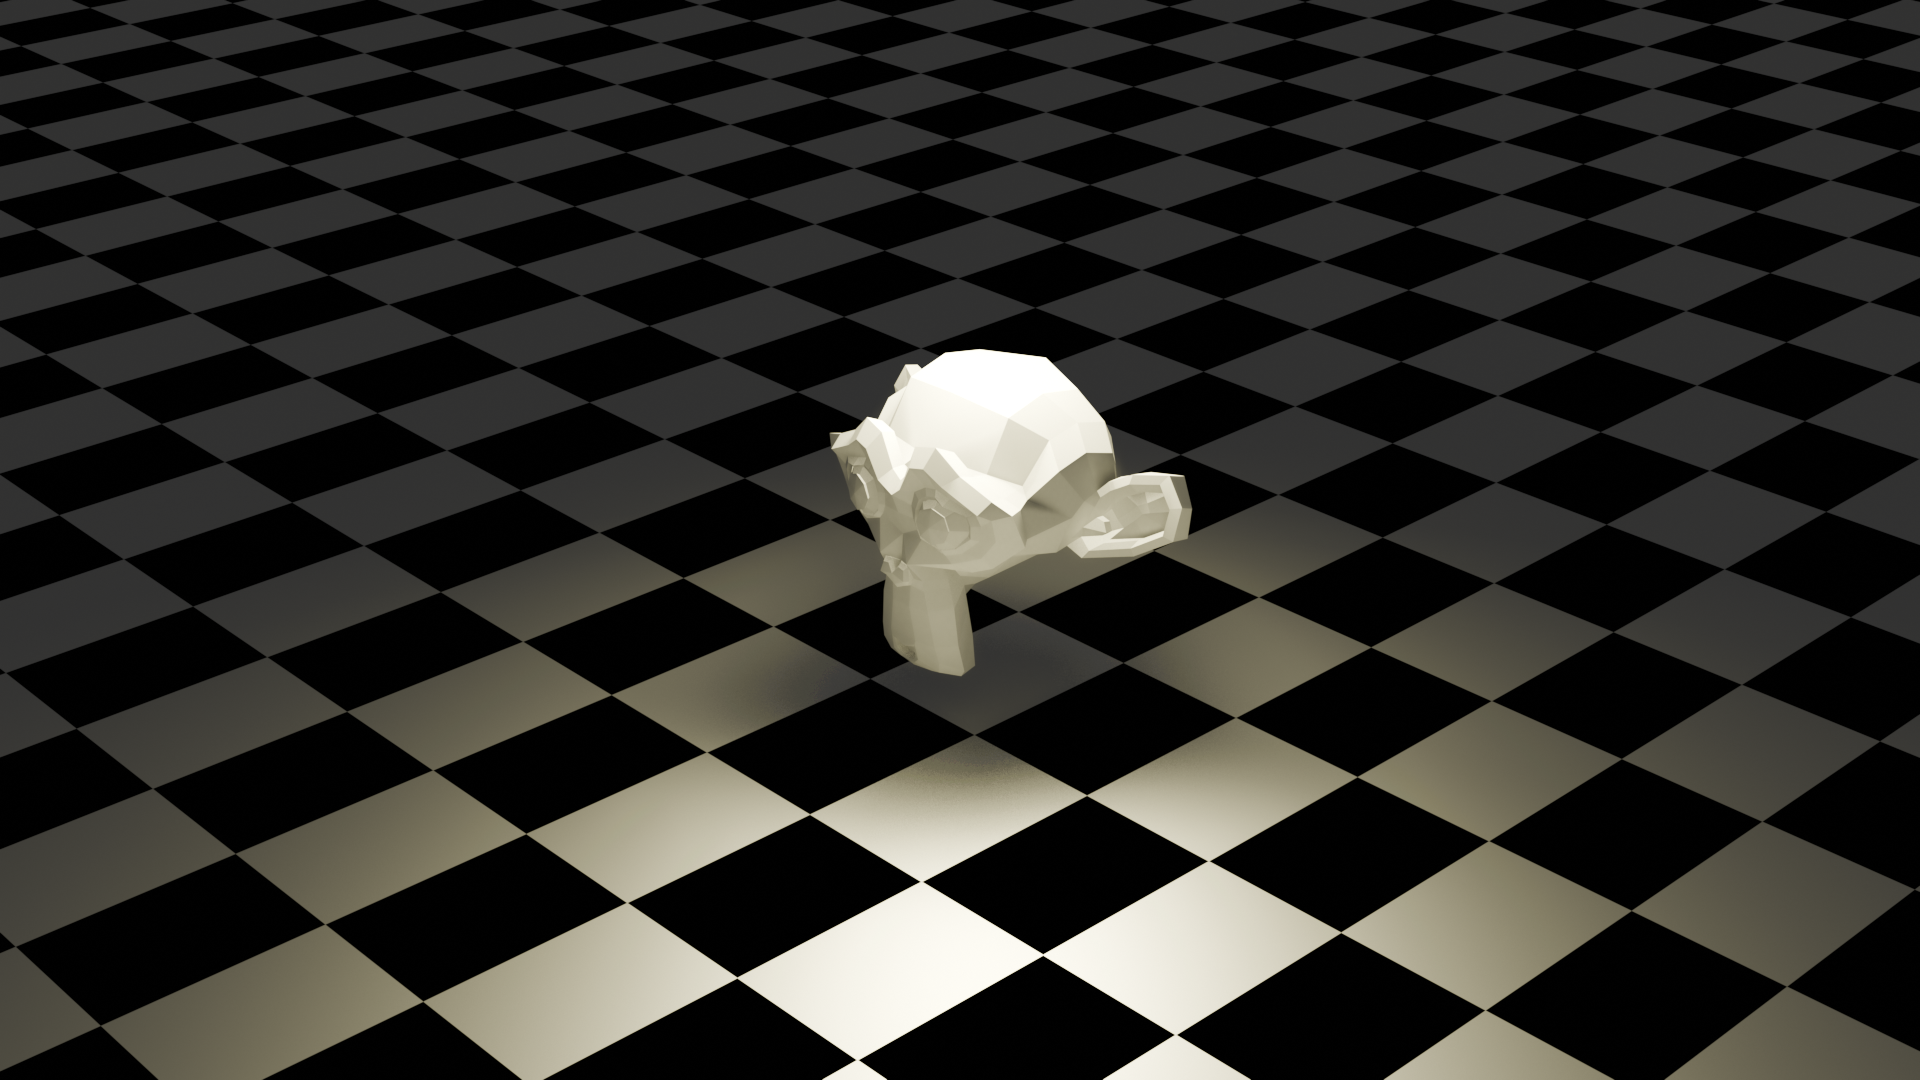
\includegraphics[width=0.5\linewidth]{images/point.png}
        \caption*{Point Light ft. Suzanne the monkey}
      \end{figure}
    \end{center}
  }
\end{frame}

\begin{frame}{Point Light Mathematics}
  \begin{columns}
    \begin{column}{0.6\textwidth}
      \begin{mathbox}{Point Light Parameters}
        \textbf{Position:} $\mathbf{P}_{\text{light}} = (x_l, y_l, z_l)$

        \textbf{Intensity:} $I_{\text{light}}$ (brightness)

        \textbf{Color:} $\mathbf{C}_{\text{light}} = (r, g, b)$

        \vspace{0.3cm}
        \pause
        \textbf{Light direction to surface point:}
        \begin{align*}
          \mathbf{L} &= \mathbf{P}_{\text{light}} - \mathbf{P}_{\text{surface}} \\
          \hat{\mathbf{L}} &= \frac{\mathbf{L}}{|\mathbf{L}|} \quad \text{(normalized)}
        \end{align*}

        \pause
        \textbf{Distance:}
        \begin{align*}
          d = |\mathbf{P}_{\text{light}} - \mathbf{P}_{\text{surface}}|
        \end{align*}
      \end{mathbox}
    \end{column}
    \begin{column}{0.4\textwidth}
      \begin{tikzpicture}[scale=0.8]
        \draw[->] (0,0) -- (3,0) node[right] {$x$};
        \draw[->] (0,0) -- (0,3) node[above] {$y$};
        \draw[->] (0,0) -- (-1,-1) node[below left] {$z$};

        \begin{scope}[plane origin={(1,1,0)},
            plane x={(0.293,1.707,0)},
            plane y={(1,1,1)},
          canvas is plane]
          \draw[ObjectColor, fill=ObjectColor!20, opacity=0.6] (0,0) circle (2);
        \end{scope}

        \node[circle, fill=LightColor, minimum size=0.6cm] (light) at (2,2.5) {};
        \node[above] at (2,3) {\footnotesize $\mathbf{P}_{\text{light}}$};

        \fill[ObjectColor] (1,1) circle (3pt);
        \node[below] at (1,0.7) {\footnotesize $\mathbf{P}_{\text{surface}}$};

        \draw[<->, thin, AccentColor] (0.8,1.2) -- (1.8,2.7)
        node[AccentColor, midway, above left] {\footnotesize $d$};

        \draw[->, ray, very thick] (1,1) -- (2,2.5);
        \node[right] at (1.7,1.9) {\footnotesize $\mathbf{L}$};

      \end{tikzpicture}
    \end{column}
  \end{columns}
\end{frame}

\begin{frame}{Attenuation}
  \begin{conceptbox}{What is Attenuation?}
    Light becomes dimmer as distance increases due to the spreading of light energy over a larger area.
    Without this effect, distant objects would appear as bright as nearby ones, which is unrealistic.
  \end{conceptbox}
  \begin{figure}
    \centering
    \begin{minipage}{0.48\textwidth}
      \centering
      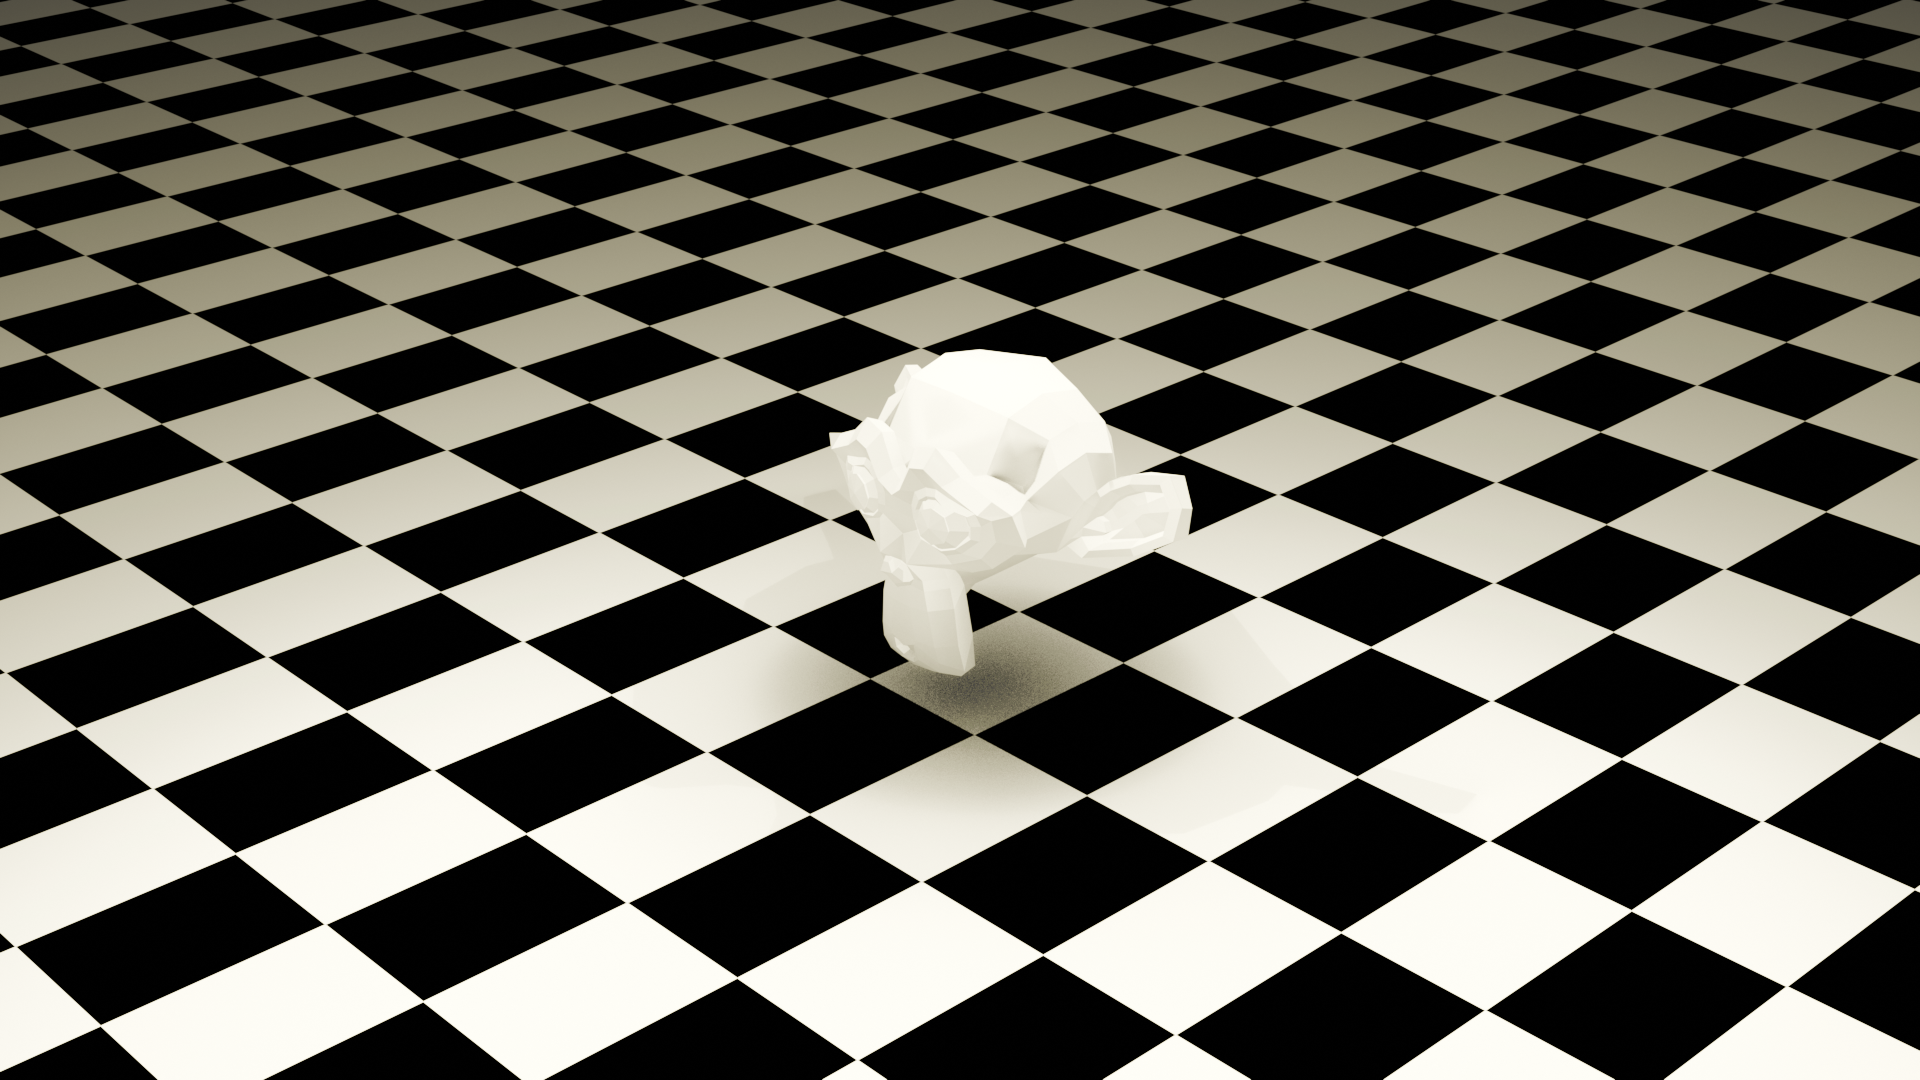
\includegraphics[width=\textwidth]{images/point_no_falloff.png}
      \caption*{No Attenuation}
    \end{minipage}
    \hfill
    \begin{minipage}{0.48\textwidth}
      \centering
      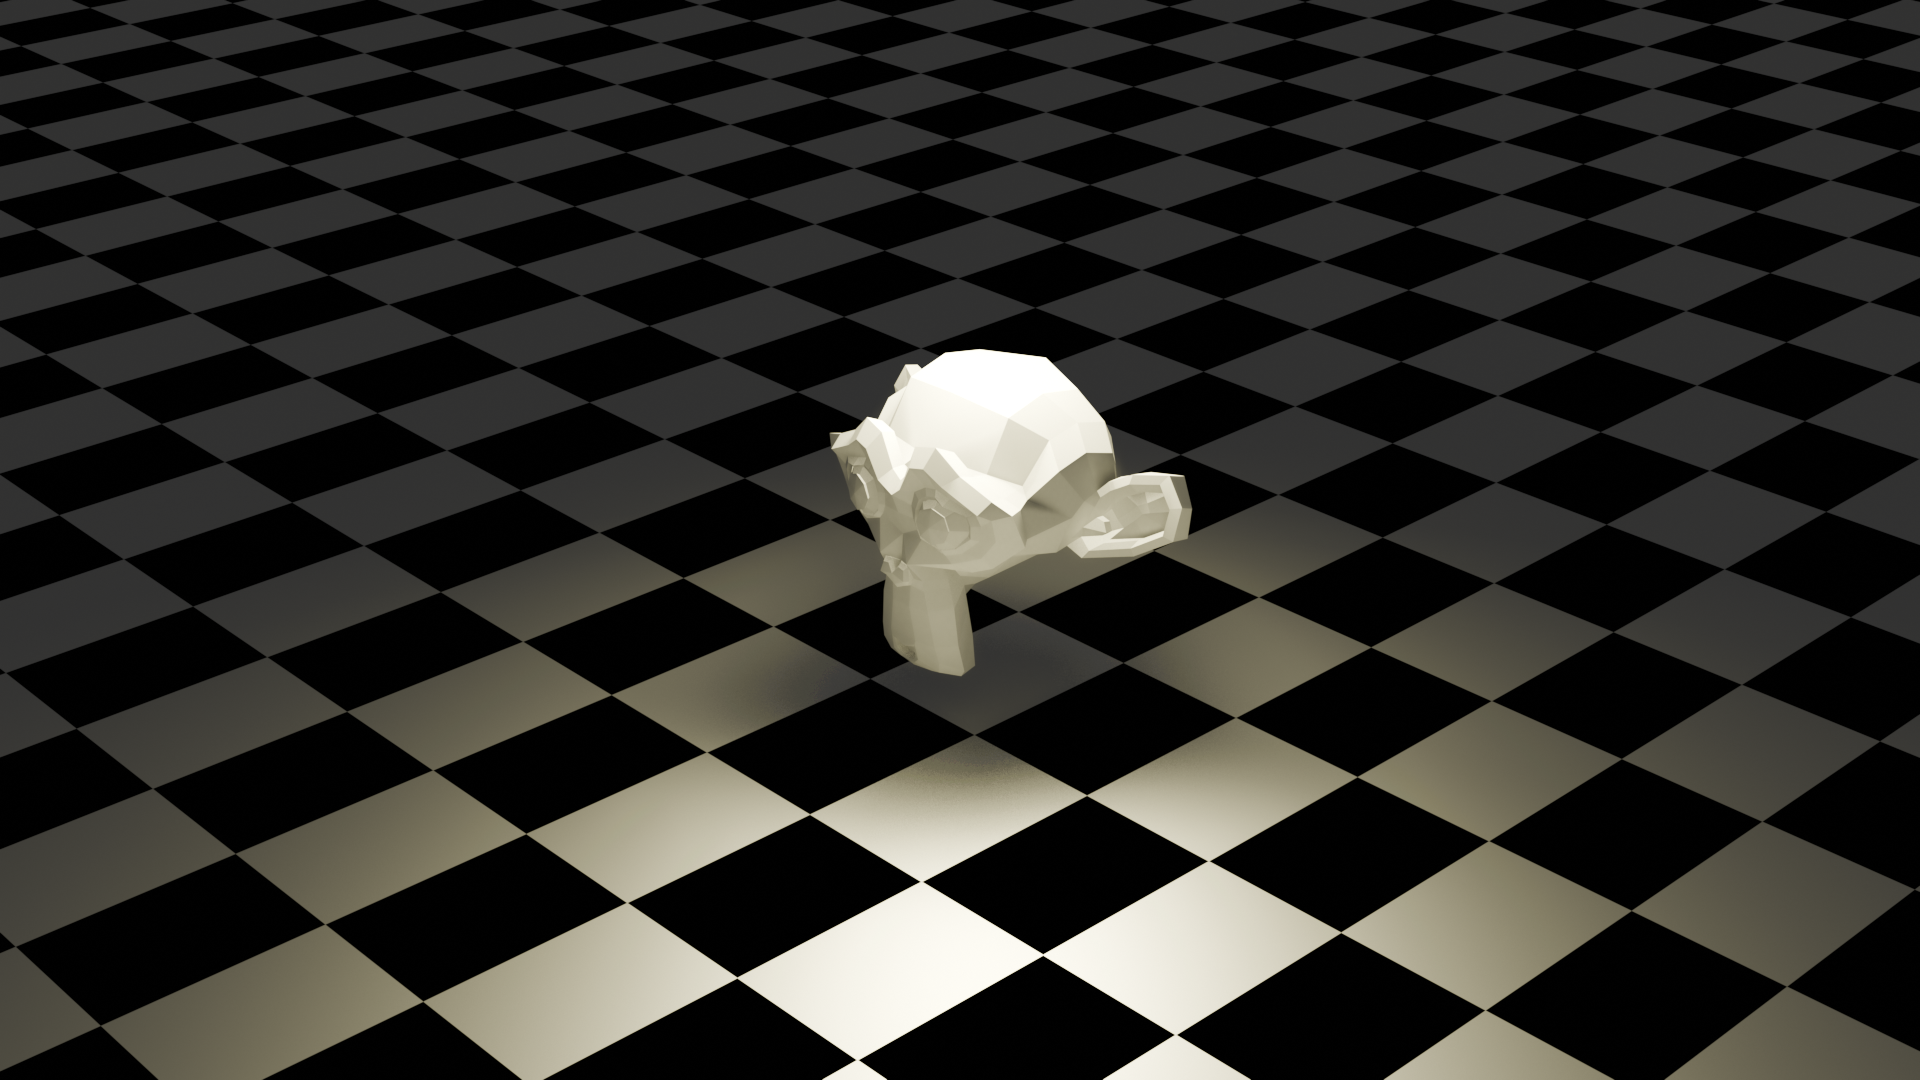
\includegraphics[width=\textwidth]{images/point.png}
      \caption*{With Attenuation}
    \end{minipage}
  \end{figure}

\end{frame}

\begin{frame}{Inverse Square Law - The Physics}
  \begin{columns}
    \begin{column}{0.6\textwidth}
      \begin{conceptbox}{$1/r^2$ Attenuation}
        \small
        \begin{itemize}
          \item \textbf{Physical principle:} Light energy spreads over larger area as distance increases.
          \item<2-> \textbf{Sphere surface area:} $A = 4\pi r^2$
          \item<3-> \textbf{Energy conservation:} Same total energy spread over larger area.
          \item<4-> \textbf{Intensity per unit area:} $I \propto \frac{1}{r^2}$
        \end{itemize}
      \end{conceptbox}

    \end{column}
    \begin{column}{0.4\textwidth}
      \begin{tikzpicture}[scale=0.6]
        % Point light
        \node[circle, fill=LightColor, minimum size=0.8cm] (light) at (0,0) {\faIcon{lightbulb}};

        % Spherical shells at different distances
        \draw[AccentColor, thick] (0,0) circle (1.5);
        \draw[AccentColor, thick] (0,0) circle (3);

        % Radius labels
        \draw[<->, thin] (0,0) -- (1.5,0) node[midway, above, xshift=0.1cm] {\footnotesize $r$};
        \draw[<->, thin] (0,0) -- (3,0) node[midway, below, xshift=0.5cm] {\footnotesize $2r$};

        % Area annotations
        \node[AccentColor] at (1.1,1.5) {\footnotesize $A_1$};
        \node[AccentColor] at (2.1,3) {\footnotesize $A_2 = 4A_1$};

        % Energy density
        \node[below] at (0,-3.5) {
          \scriptsize
          Same energy → 4× area → $\frac{1}{4}$ intensity
        };
      \end{tikzpicture}
    \end{column}
  \end{columns}

  \vspace{0.3cm}
  \only<5->{
    \begin{mathbox}{Attenuation Formula}
      \vspace*{-0.5cm}
      \begin{align*}
        I_{\text{received}} = \frac{I_{\text{light}}}{d^2} \quad \text{where } d = \text{distance to light}
      \end{align*}
    \end{mathbox}
  }
\end{frame}

\begin{frame}{Point Light Implementation}
  \begin{mathbox}{Point Light Function Structure}
    \small
    \only<1>{

      \textbf{Input parameters:}
      \begin{itemize}
        \item Light position: $\mathbf{P}_{\text{light}}$
        \item Light intensity: $I_{\text{light}}$
        \item Light color: $\mathbf{C}_{\text{light}} = (r, g, b)$
        \item Surface point: $\mathbf{P}_{\text{surface}}$
      \end{itemize}
    }
    \only<2>{

      \textbf{Calculation steps:}
      \begin{align*}
        \mathbf{L} &= \mathbf{P}_{\text{light}} - \mathbf{P}_{\text{surface}} \\
        d &= |\mathbf{L}| \\
        \hat{\mathbf{L}} &= \mathbf{L} / d \\
        I_{\text{final}} &= \frac{I_{\text{light}}}{\epsilon + d^2}
      \end{align*}
    }
  \end{mathbox}
\end{frame}